\chapter{Éléments théoriques et méthodes}

\section{Description du modèle \textbf{CROCO}}
\textbf{CROCO} est un modèle de résolution numérique des océans permettant des études sur des zones côtières ou hauturières. Il s'agit d'un modèle parent du modèle \textbf{ROMS}, utilisant des scripts Fortran compilés en C prenant en entrée des fichiers netcdf et qui produit des fichiers de sortie netcdf également. Ces scripts sont compatibles avec les modules de parallélisation permettant une résolution plus rapide par fragmentation de la grille. Dans notre cas nous effectuerons les simulations sur le cluster du CINES Adastra ce qui nous permet de faire des simulations de plusieurs sur la zone étudiée, ainsi que des ensembles de simulations, que nous décrirons plus tard.

\subsection{Grille et équations}
\subsubsection{Résolution verticale}
\begin{wrapfigure}{r}{0.4\textwidth}
    \centering
    \vspace{-60pt}
    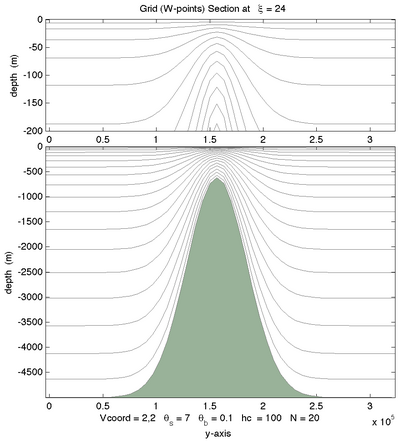
\includegraphics[width=0.4\textwidth]{figures/vcoord_ex4.png}
    \caption{Exemple de résolution verticale tiré de la documentation de \textbf{CROCO} - ROMS-RUTGERS team}
    \label{fig:vcoord_ex4}
    \vspace{-50pt}
\end{wrapfigure}

La particularité de \textbf{CROCO} est l'emploi d'une coordonnée d'étirement verticale qui suit le relief du terrain, la coordonnée $\sigma$, qui varie entre $-1$ et $0$. Cette approche va permettre une meilleure résolution des phénomènes côtiers ou à faible profondeur, tout en évitant de surcharger le modèle avec une grille trop résolue verticalement. Cela nous permet de réécrire la coordonnée verticale $z$ en \autoref{eq:1}
\begin{subequations} \label{eq:1}
    \begin{align}
        z(x,y,\sigma,t)  = & z_0(x,y,\sigma) + \zeta(x,y,t) \left[ 1+\frac{z_0(x,y,\sigma)}{h(x,y)} \right] \label{eq:1a} \\
        z_0 (x,y,\sigma) = & h_c \sigma +    \left[ h(x,y) - h_c \right]  Cs(\sigma) \label{eq:1b}
    \end{align}
\end{subequations}

Ici, $z_0(x,y,\sigma)$ est une transformation verticale non-linéaire, $\zeta(x,y,t)$ et $h(x,y)$ sont respectivement la surface libre et le fond de l'océan, $h_c$ est la profondeur de transition entre les niveaux de surface horizontaux et les niveaux de profondeur qui suivent la bathymétrie (le relief) et $Cs(\sigma)$ est un étirement non dimensionnel, vertical et monotone. 

$Cs(\sigma)$ est défini avec deux autres paramètres, $\theta_s$ le paramètre d'étirement de surface et $\theta_b$ le paramètre d'étirement de fond. Dans notre cas, $Cs(\sigma)$ suivra la loi en \autoref{eq:Cs}.
\begin{equation} \label{eq:Cs}
	Cs(\sigma) = (1-\theta_b) \frac{\sinh(\theta_s \ \sigma)}{\sinh(\theta_s)}
+ \theta_b \left[  \frac{0.5 \ \tanh\left( \left(\sigma+0.5 \right)\theta_s \right)  }{ \tanh (0.5 \ \theta_s) }  - 0.5 \right]
\end{equation}

On peut voir en \autoref{fig:vcoord_ex4} l'avantage que procure cette résolution variables dans les zones a faible profondeur. Si nous n'avions pas cette résolution, nous ne pourrions pas simuler correctement les phénomènes apparaissant dans ces zones dite \textit{shallow waterss} (eaux peu profondes). Toutes ces expressions sont gérées au sein de \textbf{CROCO}, nous donnons juste en entrée les différents paramètres que nous souhaitons. Vous trouverez en annexe d'autres exemples de configuration en \autoref{sec:vertical grid}.

\subsubsection{Grille horizontale}
Dans le cas de simulation à grande échelle des océans, il n'est plus possible d'utiliser les simples coordonnées $x$ et $y$ formant un repère orthonormé, il est nécessaire de prendre en compte la courbure de la Terre ce qui introduit deux nouvelles coordonnées $\xi$ et $\eta$, alignées respectivement selon la latitude et la longitude, ainsi que la métrique terrestre que nous allons définir avec $m$ et $n$. On peut donc écrire les relations entre la longueur d'un arc horizontal $ds$ et les distances différentielles $d\xi$ et $d\eta$
\begin{subequations} \label{eq:ds}
	\begin{align}
		(ds)_\xi = \left( \frac{1}{m} \right) d\xi && (ds)_\eta = \left( \frac{1}{n} \right) d\eta
	\end{align}
\end{subequations}

\begin{wrapfigure}{r}{0.4\textwidth}	
\centering
	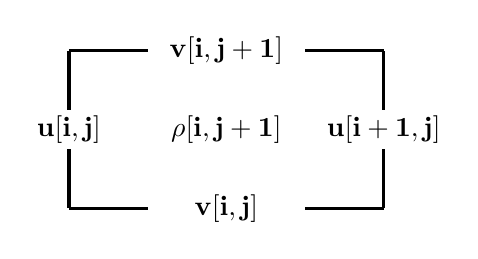
\begin{tikzpicture}
	\draw[very thick] (0,0) -- (1,0);
	\node at (2,0) {$\mathbf{v\boldsymbol{[}i,j\boldsymbol{]}}$};
	\draw[very thick] (3,0) -- (4,0);
	
	\draw[very thick] (0,0) -- (0,0.75);
	\node at (0,1) {$\mathbf{u\boldsymbol{[}i,j\boldsymbol{]}}$};
	\draw[very thick] (0,1.25) -- (0,2);
	
	\draw[very thick] (0,2) -- (1,2);
	\node at (2,2) {$\mathbf{v\boldsymbol{[}i,j+1\boldsymbol{]}}$};
	\draw[very thick] (3,2) -- (4,2);
	
	\draw[very thick] (4,0) -- (4,0.75);
	\node at (4,1) {$\mathbf{u\boldsymbol{[}i+1,j\boldsymbol{]}}$};
	\draw[very thick] (4,1.25) -- (4,2);
	
	\node at (2,1) {$\mathbf{\boldsymbol{\rho} \boldsymbol{[}i,j+1\boldsymbol{]}}$};
	\end{tikzpicture}
	\caption{Décalage des variables sur la grille utilisée par \textbf{CROCO}}
	\vspace{-30pt}
\end{wrapfigure}

\subsubsection{Grille décalée}
La discrétisation au sein de \textbf{CROCO} est basée sur une grille décalée (\textit{staggered grid} en anglais). Les données comme la surface libre $\zeta$, la densité $\rho$ ainsi que les traceurs telles que la température $T$ ou la salinité $S$ seront localisés au milieu de chaque cellule alors que les vitesses horizontales $(u,v)$ se trouveront sur les bords des cellules. On voit donc que si l'on souhaite paralléliser notre simulation, ce que nous allons faire, il est nécessaire de diviser notre domaine entier d'une certaine manière: Les premiers sous-domaines, ou boîte, simulés à chaque itération de temps vont être ceux situés en bas à gauche de notre domaine.



